\chapter{Kubernetes}
\section{¿Por qué existe Kubernetes?}
Kubernetes es una plataforma de código abierto que gestiona contenedores y automatiza sus recursos (almacenamiento, red y seguridad), asegurando que las aplicaciones funcionen siempre en el estado deseado.

A diferencia de las herramientas de infraestructura DevOps tradicionales que 
requieren una gestión manual, Kubernetes destaca por la reproducibilidad de la
 infraestructura. En el DevOps moderno, solucionar un problema de forma manual en un solo componente
  genera inconsistencias. Kubernetes evita esto automatizando la réplica exacta de los componentes en 
  todo el sistema, lo que reduce los fallos y optimiza la administración en los centros de datos.
\subsection{Repaso de algunos términos clave antes de empezar}
El texto define los conceptos fundamentales para entender el ecosistema de Kubernetes:

\subsection{Componentes de la Arquitectura}
\begin{itemize}
    \item \textbf{Control plane (Plano de control):} El ``cerebro'' del clúster (a veces denominado \textit{Masters}). Se encarga de programar los contenedores y gestionar todos los objetos de Kubernetes.
    \item \textbf{Node (Nodo):} Una máquina que ejecuta el proceso \texttt{kubelet}.
    \item \textbf{kubelet:} El agente de Kubernetes que corre en los nodos del clúster. Hace lo que el plano de control le ordena.
    \item \textbf{kubectl:} La herramienta de línea de comandos para comunicarse con el plano de control de Kubernetes.
\end{itemize}

\subsubsection{Contenedores y Despliegue}
\begin{itemize}
    \item \textbf{Container (Contenedor):} Una imagen Docker u OCI que típicamente ejecuta una aplicación.
    \item \textbf{OCI (Open Container Initiative):} El formato común de imagen para construir aplicaciones ejecutables y autónomas. También conocido como imágenes Docker.
    \item \textbf{Pod:} El objeto de Kubernetes que encapsula un contenedor en ejecución.
    \item \textbf{Deployment (Despliegue):} Una colección de Pods que es gestionada por Kubernetes.
    \item \textbf{DaemonSet:} Al igual que un \textit{deployment}, pero se ejecuta en cada nodo de un clúster.
\end{itemize}

\subsubsection{Interfaces}
\begin{itemize}
    \item \textbf{CNI y CSI:} Las interfaces de red y almacenamiento de contenedores (\textit{Container Networking Interface} y \textit{Container Storage Interface}, respectivamente) que permiten red y almacenamiento acoplables (\textit{pluggable}) para los Pods que corren en Kubernetes.
\end{itemize}

\subsection{El problema del desvío de infraestructura (Infrastructure Drift) y Kubernetes}

La gestión de la infraestructura de manera reproducible implica controlar el \textbf{infrastructure drift}
 (desvío de configuración), el cual ocurre a medida que el hardware, las normativas de cumplimiento 
 y los requisitos del centro de datos cambian con el tiempo. Esto afecta tanto a la definición de las 
 aplicaciones como a la administración de los hosts donde se ejecutan. 

Los ingenieros de TI suelen enfrentarse constantemente a tareas repetitivas y tediosas (\textit{toil}) como:
\begin{itemize}
    \item Actualizar la versión de Java en una flota entera de servidores.
    \item Asegurar que ciertas aplicaciones no se ejecuten en ubicaciones específicas.
    \item Reemplazar o escalar hardware antiguo o dañado, migrando las aplicaciones fuera de él.
    \item Gestionar manualmente las rutas de balanceo de carga.
    \item Olvidar documentar los nuevos cambios en la infraestructura debido a la falta de un lenguaje de configuración común y obligatorio.
\end{itemize}

A medida que se actualizan los servidores en la nube o en un centro de datos 
local, aumenta la probabilidad de que su estado real se desvíe de la arquitectura de TI planificada, provocando que las aplicaciones corran en lugares incorrectos, con asignaciones de recursos erróneas o con accesos a módulos de almacenamiento equivocados.

\subsubsection{Soluciones y evolución tecnológica}
Kubernetes permite centralizar la gestión de todo el espacio de estados de las
 aplicaciones mediante \texttt{kubectl}, un cliente de línea de comandos que realiza llamadas REST al servidor de la API de Kubernetes, o mediante clientes programáticos. 

A diferencia de tecnologías previas como \textit{Puppet, Chef, Mesos, Ansible} o \textit{SaltStack}:
\begin{itemize}
    \item Kubernetes hereda las capacidades de gestión de estado de herramientas como 
    \textit{Puppet} y los conceptos de programación de aplicaciones de \textit{Mesos}.
    \item Mientras que \textit{Ansible, SaltStack} y \textit{Terraform} se encargan de la 
    configuración inicial del sistema operativo (como cortafuegos o instalación de binarios), Kubernetes
     gestiona estos conceptos utilizando \textbf{contenedores privilegiados} en entornos Linux 
     (conocidos como \textit{HostProcess Pods} en Windows). Un ejemplo de esto es el componente 
     \texttt{kube-proxy}, que maneja las reglas de \texttt{iptables} para enrutar el tráfico de red.
\end{itemize}

Finalmente, grandes compañías como Google, Microsoft, Amazon y VMware han adoptado la 
contenedorización como una estrategia clave para ejecutar miles de aplicaciones en entornos de 
nube y \textit{bare metal}, convirtiendo a Kubernetes en el estándar moderno indiscutible para la orquestación de contenedores.


\subsection{Contenedores e imágenes}

Las aplicaciones tienen dependencias que deben ser cubiertas por el host donde se 
ejecutan. En la era previa a los contenedores, los desarrolladores lograban esto de manera improvisada (por ejemplo, una aplicación Java requería una JVM en ejecución junto con reglas de cortafuegos para comunicarse con una base de datos).

En su esencia, Docker puede entenderse como una forma de ejecutar contenedores, 
donde un \textbf{contenedor} es una imagen OCI (\textit{Open Container Initiative}) 
en ejecución. La especificación OCI es un estándar para definir una imagen ejecutable por programas como Docker, y consiste básicamente en un archivo \textit{tarball} con varias capas. Cada una de estas capas contiene elementos como binarios de Linux y archivos de la aplicación. Así, al ejecutar un contenedor, el \textit{runtime} (como Docker, containerd o CRI-O) toma la imagen, la desempaqueta y arranca un proceso en el sistema host con el contenido de dicha imagen.

Los contenedores añaden una capa de aislamiento que elimina la necesidad de gestionar librerías 
en un servidor o precargar la infraestructura con otras dependencias accidentales. Por ejemplo, si se tienen dos aplicaciones Ruby que requieren versiones diferentes de la misma librería, se pueden utilizar dos contenedores independientes. Cada aplicación queda aislada con la versión específica que necesita. Esto soluciona la famosa frase: \textit{``Bueno, en mi máquina funciona''}. El uso de imágenes simplifica la ejecución del mismo software en diferentes servidores.

% --- CÓDIGO PARA INSERTAR LA IMAGEN (Ajusta el nombre del archivo) ---
\begin{figure}[htbp]
    \centering
    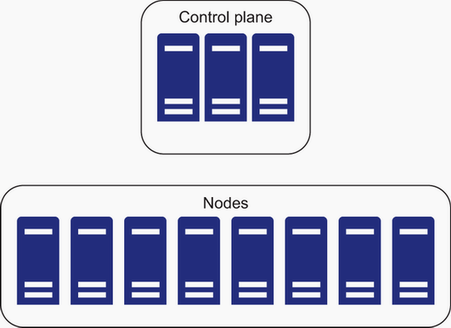
\includegraphics[width=0.8\textwidth]{capitulos/img/image1.png} % Cambia esto por el nombre de tu archivo de imagen
    \caption{Aislamiento de dependencias mediante contenedores (Figura 1.1).}
    \label{fig:aislamiento_contenedores}
\end{figure}
% -----------------------------------------------------------------

Al combinar el uso de imágenes con Kubernetes se obtienen servidores 
inmutables y una simplicidad de nivel empresarial. Como los contenedores se están convirtiendo rápidamente en el estándar de la industria para 
el despliegue de software, vale la pena mencionar algunos datos:

\begin{itemize}
    \item En una encuesta realizada a más de 88,000 desarrolladores, 
    Docker y Kubernetes ocuparon el tercer lugar entre las tecnologías de desarrollo más queridas en 2020, justo detrás de Linux y Docker solo.
    \item Datadog descubrió recientemente que Docker abarca el 50\% o 
    más del flujo de trabajo del desarrollador promedio. Asimismo, la adopción a nivel corporativo supera el 25\% de todas las empresas.
\end{itemize}

En conclusión, la necesidad de automatizar los contenedores es el lugar 
exacto donde encaja Kubernetes. Esta plataforma domina su sector de la misma 
manera que lo hicieron la base de datos Oracle y la plataforma de virtualización vSphere en sus mejores momentos. Se predice para Kubernetes una 
longevidad similar a la de esas tecnologías. 

El propósito de este libro es llevarte más allá de los principios básicos 
hacia el núcleo de bajo nivel. Comencemos analizando un flujo de trabajo de Kubernetes extremadamente simplificado que demuestra algunos de los
 principios de nivel superior para construir y ejecutar microservicios.

\subsection{Fundamentos esenciales de Kubernetes (Core foundation of Kubernetes)}

En su núcleo, todo en Kubernetes se define mediante archivos de texto plano utilizando \textbf{YAML} o \textbf{JSON}. A través de este enfoque declarativo, la plataforma ejecuta imágenes OCI y permite configurar reglas de red, autenticación y autorización basada en roles (RBAC), entre otros recursos. Al aprender esta sintaxis única y su estructura, es posible configurar, gestionar y optimizar cualquier sistema de Kubernetes.

\subsubsection{Flujo de trabajo y construcción de imágenes}
Para ilustrar el despliegue de una arquitectura de microservicios básica (por ejemplo, un servidor MySQL y un cliente personalizado en Python), el proceso comienza con la definición de sus respectivos archivos \texttt{Dockerfile}:

% Dockerfile de MySQL
\begin{verbatim}
# Servidor MySQL
FROM alpine:3.15.4
RUN apk add --no-cache mysql
ENTRYPOINT ["/usr/bin/mysqld"]
\end{verbatim}

% Dockerfile del Cliente Python
\begin{verbatim}
# Cliente personalizado en Python
FROM python:3.7
WORKDIR /myapp
COPY src/requirements.txt ./
RUN pip install -r requirements.txt
COPY src /myapp
CMD [ "python", "mysql-custom-client.py" ]
\end{verbatim}

Típicamente, estas imágenes se construyen (\texttt{docker build}) y se suben (\texttt{docker push}) a un registro OCI (ya sea uno privado como \textit{Harbor} o uno público como \textit{Docker Hub}) para que los nodos del clúster puedan descargarlas durante el tiempo de ejecución.

\subsubsection{Definición y despliegue en Kubernetes}
Para ejecutar estas aplicaciones como contenedores dentro de Kubernetes, se encapsulan en objetos llamados \textbf{Pods}. La definición se realiza en un único archivo YAML (por ejemplo, \texttt{my-app.yaml}):

\begin{verbatim}
apiVersion: v1
kind: Pod
metadata:
  name: core-k8s
spec:
  containers:
    - name: my-mysql-server
      image: myregistry.com/mysql-server:v1.0
---
apiVersion: v1
kind: Pod
metadata:
  name: core-k8s-mysql
spec:
  containers:
    - name: my-sqlclient
      image: myregistry.com/mysql-custom-client:v1.0
      command: ['tail','-f','/dev/null']
\end{verbatim}

Este archivo se envía al servidor de la API de Kubernetes ejecutando el comando \texttt{kubectl create -f my-app.yaml}. El plano de control almacena la definición y se encarga de que ambos Pods se programen y ejecuten en algún lugar del clúster.

\subsubsection{Consistencia eventual y escalabilidad}
Este proceso de despliegue no es instantáneo. Requiere que los nodos del clúster respondan a los eventos y actualicen su estado mediante el agente \texttt{kubelet}, el cual se comunica constantemente con la API. Debido a que las imágenes deben descargarse y pueden ocurrir fallos en el camino, Kubernetes se diseña bajo un modelo de \textbf{consistencia eventual} (\textit{eventually consistent system}). En lugar de garantizar una consistencia inmediata, el sistema trabaja continuamente en la \textbf{reconciliación} para llevar el estado real del clúster hacia el estado deseado que el usuario ha solicitado.

Este modelo declarativo escala de forma natural a escenarios de producción complejos. Si se solicita desplegar cinco instancias de una aplicación distribuidas en tres zonas de disponibilidad de la nube, Kubernetes se encarga de la logística de la programación. Al delegar la implementación interna y el mantenimiento del estado a la propia plataforma, se elimina casi por completo la necesidad de realizar actualizaciones manuales o personalizadas con herramientas como \textit{Ansible} o \textit{Puppet} en entornos de producción.

\begin{itemize}
    \item \textbf{Gestión integral de la infraestructura mediante YAML:} Kubernetes automatiza todos los aspectos de la pila tecnológica a través de su API, permitiendo definir las reglas tradicionales de TI como recursos de texto plano. Esto incluye:
    \begin{itemize}
        \item Configuración de servidores, puertos y rutas IP.
        \item Disponibilidad de almacenamiento persistente para las aplicaciones.
        \item Alojamiento de \textit{software} en servidores específicos o arbitrarios.
        \item Aprovisionamiento de seguridad (como RBAC o reglas de red para la comunicación entre aplicaciones).
        \item Configuración de DNS tanto a nivel global como por aplicación.
    \end{itemize}
    Todos estos componentes se representan como objetos dentro de la API de Kubernetes. La plataforma aplica los cambios, los monitorea y resuelve las interrupciones o fallos momentáneos de forma automática hasta alcanzar el estado final deseado. Al delegar esta automatización, se mitigan los incidentes imprevistos sin intervención manual directa, permitiendo que el equipo de DevOps se enfoque en resolver problemas complejos, planificar a futuro y encontrar soluciones óptimas para el negocio.
\end{itemize}

\subsection{Características principales de Kubernetes (Kubernetes features)}

Las plataformas de orquestación de contenedores permiten a los desarrolladores automatizar la ejecución de instancias, el aprovisionamiento de hosts y la extensión del ciclo de vida de las aplicaciones. Esencialmente, los contenedores necesitan Pods y los Pods necesitan a Kubernetes para cumplir con las siguientes funciones esenciales:

\begin{itemize}
    \item \textbf{API agnóstica de la nube:} Expone una API unificada y neutral respecto al proveedor de nube a través del \textit{API server}.
    \item \textbf{Integración nativa:} Se integra con las principales plataformas de nube e hipervisores mediante el \textit{Kubernetes Controller Manager} (KCM).
    \item \textbf{Tolerancia a fallos:} Proporciona un marco resiliente para almacenar y definir el estado de los servicios, aplicaciones y configuraciones.
    \item \textbf{Gestión de despliegues:} Minimiza el tiempo de inactividad de cara al usuario durante las actualizaciones de hosts o aplicaciones mediante estrategias como los \textit{rolling updates}.
    \item \textbf{Escalado automático y balanceo de carga:} Automatiza el escalado de hosts y aplicaciones, y crea integraciones de red internas y externas con balanceo de carga (\textit{Service types: ClusterIP, NodePort} o \textit{LoadBalancer}).
    \item \textbf{Programación inteligente:} El \textit{Kubernetes scheduler} programa las aplicaciones en hardware virtualizado específico basándose en metadatos y etiquetas de nodo (\textit{node labeling}).
    \item \textbf{Alta disponibilidad y tareas por lotes:} Garantiza que ciertos contenedores corran en todos los nodos mediante \textit{DaemonSets} y permite ejecutar procesos por lotes (\textit{Jobs}).
    \item \textbf{Descubrimiento de servicios:} Permite la resolución de nombres DNS mediante la integración nativa de \textit{CoreDNS} con el servidor de la API.
    \item \textbf{Extensibilidad de la API:} Permite construir programas nativos basados en la API utilizando Definiciones de Recursos Personalizados (\textit{CRDs}).
    \item \textbf{Inspección y depuración:} Facilita la auditoría de procesos fallidos y la ejecución remota dentro de los contenedores mediante comandos como \texttt{kubectl exec} y \texttt{kubectl describe}.
    \item \textbf{Gestión de almacenamiento:} Permite montar almacenamiento local o remoto y gestionar volúmenes declarativos con las API de \textit{StorageClass} y \textit{PersistentVolumes}.
\end{itemize}

% --- CÓDIGO PARA INSERTAR LA IMAGEN DEL CLÚSTER (Figura 1.2) ---
\begin{figure}[htbp]
    \centering
    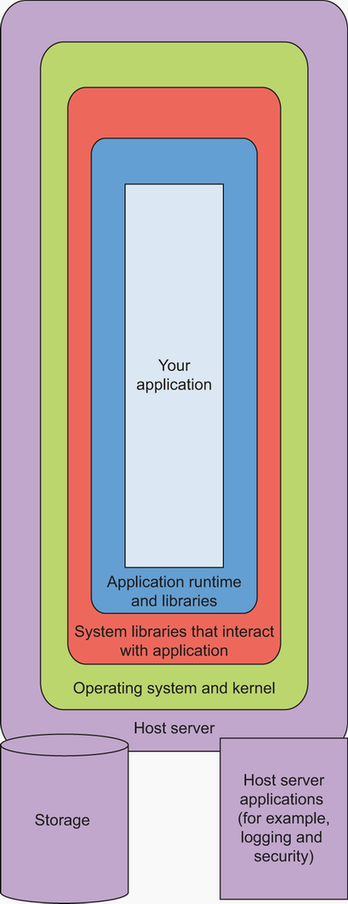
\includegraphics[width=0.85\textwidth]{capitulos/img/image2.png} % Cambia esto por el nombre de tu archivo de imagen
    \caption{Diagrama simplificado de la arquitectura de un clúster de Kubernetes (Figura 1.2).}
    \label{fig:kubernetes_cluster}
\end{figure}
% ---------------------------------------------------------------

La base de Kubernetes es un clúster compuesto por nodos. Aunque su complejidad suele ser una de las quejas más comunes entre los ingenieros, la plataforma resuelve un problema inherentemente complejo de estandarización y ciclo de vida que, de otro modo, sería muy difícil de solucionar.

\subsubsection{Escenario típico de fallo y resiliencia}
Si una organización no requiere alta disponibilidad, escalabilidad u orquestación, tal vez no necesite Kubernetes. Para entender su valor bajo presión, consideremos un escenario típico de fallo:
\begin{enumerate}
    \item Un nodo deja de responder al plano de control (\textit{control plane}).
    \item El plano de control reprograma automáticamente los Pods que corrían en el nodo afectado hacia otros nodos operativos.
    \item Cuando un usuario consulta el estado mediante \texttt{kubectl}, el \textit{API server} responde con la información corregida sobre el nodo caído y la nueva ubicación de los Pods.
    \item Todo el tráfico de los clientes hacia el servicio del Pod se redirige automáticamente a la nueva ubicación.
    \item Los volúmenes de almacenamiento persistente conectados a los Pods del nodo fallido se reasignan a la nueva ubicación del Pod para mantener la lectura de los datos previos.
\end{enumerate}

\subsubsection{El ecosistema y sistemas operativos inmutables}
Bajo el capó, Kubernetes se apoya fuertemente en cientos de tecnologías de la pila de Linux. Por ello, 
resulta natural ejecutar Kubernetes sobre \textbf{sistemas operativos inmutables}, donde el SO base solo
 se actualiza por completo y en bloque, aportando ventajas críticas de estabilidad.

Kubernetes ofrece la flexibilidad de ejecutarse en la nube, en servidores físicos (\textit{bare metal}), 
en una \textit{Raspberry Pi}, en superordenadores/mainframes de última generación (como IBM PowerPC) e
 incluso en entornos críticos de defensa aeroespacial. A medida que el ecosistema \textit{cloud native} madura, permite a
  las organizaciones adoptar mejores prácticas, prevenir problemas de manera proactiva y mantener la consistencia del 
  entorno para evitar el \textit{drift} (desvío de configuración) tecnológico.


\subsection{Componentes y arquitectura de Kubernetes (Kubernetes components and architecture)}

A alto nivel, la arquitectura de Kubernetes está compuesta por la infraestructura física o 
virtual (el hardware) y la división de este hardware para ejecutar tanto el plano de control como los nodos de trabajo (\textit{worker nodes}):

\begin{itemize}
    \item \textbf{Infraestructura de hardware (Hardware infrastructure):} Incluye las computadoras (servidores), la infraestructura de red, los sistemas de almacenamiento y el registro de contenedores (\textit{container registry}).
    \item \textbf{Nodos de trabajo de Kubernetes (Kubernetes worker nodes):} Representan la unidad básica de cómputo dentro de un clúster de Kubernetes, encargados de ejecutar los contenedores de las aplicaciones.
    \item \textbf{Plano de control de Kubernetes (Kubernetes control plane):} Es la ``nave nodriza'' de Kubernetes. Este componente engloba el servidor de la API (\textit{API server}), el programador (\textit{scheduler}), el administrador de controladores (\textit{controller manager}) y otros controladores internos encargados de mantener el estado global del sistema.
\end{itemize}

% --- CÓDIGO PARA INSERTAR LA IMAGEN DE LA ARQUITECTURA (Figura 1.3) ---
\begin{figure}[htbp]
    \centering
    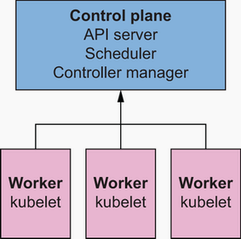
\includegraphics[width=0.9\textwidth]{capitulos/img/image3.png} % Cambia esto por el nombre de tu archivo de imagen
    \caption{Arquitectura general de Kubernetes: Infraestructura, Plano de Control y Nodos de Trabajo (Figura 1.3).}
    \label{fig:kubernetes_architecture}
\end{figure}
% ---------------------------------------------------------------------

\subsection{La API de Kubernetes (The Kubernetes API)}

El aspecto fundamental para administrar microservices y aplicaciones contenedorizadas en Kubernetes consiste simplemente en declarar objetos de su API; la plataforma se encarga de gestionar el resto de forma automática. Casi cualquier acción ejecutada a través de \texttt{kubectl} se traduce en una operación de lectura o escritura en un objeto definido y versionado dentro del servidor de la API (\textit{API server}), el cual almacena los datos en su componente de persistencia, \texttt{etcd}.

El \texttt{kube-apiserver} expone una interfaz RESTful que permite realizar operaciones CRUD (crear, leer, actualizar y eliminar) sobre todos los recursos del sistema. Por lo general, todo objeto de la API de Kubernetes cuenta con tres elementos esenciales:
\begin{itemize}
    \item Un nombre de versión de la API (\textit{API version}, por ejemplo: \texttt{v1} o \texttt{rbac.authorization.k8s.io/v1}).
    \item Un tipo de recurso (\textit{kind}, por ejemplo: \texttt{kind: Deployment}).
    \item Una sección de metadatos (\textit{metadata}).
\end{itemize}

Este robusto esquema de versionado de API (diseñado originalmente por Brian Grant, uno de los fundadores de Kubernetes) facilita las actualizaciones del sistema y define contratos claros para el ciclo de vida de los recursos en sus fases \textit{Alpha, Beta} y \textit{GA} (Disponibilidad General).

\subsubsection{Tipos de recursos y Namespaces}
En un clúster estándar de Kubernetes existen alrededor de 70 tipos de API distintos. Estos recursos se pueden consultar mediante el comando \texttt{kubectl api-resources}, el cual devuelve un listado con la siguiente estructura:

\begin{verbatim}
$ kubectl api-resources | head
NAME                    SHORTNAMES  NAMESPACED  KIND
bindings                            true        Binding
componentstatuses       cs          false       ComponentStatus
configmaps              cm          true        ConfigMap
endpoints               ep          true        Endpoint
events                  ev          true        Event
limitranges             limits      true        LimitRange
namespaces              ns          false       Namespace
nodes                   no          false       Node
persistentvolumeclaims  pvc         true        PersistentVolumeClaim
\end{verbatim}

Como se observa en la salida, cada recurso de la API posee un nombre corto (\textit{short name}), un nombre completo y un indicador booleano (\textit{NAMESPACED}) que determina si el objeto está restringido o no a un \textbf{Namespace}.

Los \textbf{Namespaces} (Espacios de nombres) proporcionan una agrupación jerárquica y lógica para los recursos. Al desplegar una aplicación compuesta por múltiples microservicios, es una práctica común crear todos sus Pods, Services y \textit{PersistentVolumeClaims} (PVCs) dentro de un mismo Namespace. Esto simplifica el aislamiento y permite que, al momento de retirar la aplicación, baste con eliminar dicho Namespace para limpiar de forma limpia y ordenada todos los objetos asociados.

\subsection{Ejemplo uno: Un minorista en línea (Example one: An online retailer)}

Imaginemos un gran comercio minorista en línea que necesita escalar rápidamente para responder a la demanda estacional, como ocurre durante las vacaciones o festividades. Históricamente, predecir la demanda y escalar la infraestructura para soportarla ha sido uno de sus mayores desafíos. 

Kubernetes resuelve la multitud de problemas asociados a la ejecución de sistemas distribuidos, altamente disponibles y escalables. No solo representa una mejor estrategia para operar el negocio, sino que constituye la plataforma más eficiente y efectiva para la gestión de sistemas. 

Al combinar el potencial de Kubernetes con los proveedores de servicios en la nube, es posible ejecutar cargas de trabajo en servidores de terceros únicamente cuando se requieren recursos adicionales. Esto elimina por completo la necesidad de comprar, configurar y mantener hardware costoso que de otro modo permanecería inactivo la mayor parte del año.

\subsection{Ejemplo dos: Una solución de donaciones en línea (Example two: An online giving solution)}

Consideremos el caso de un sitio web de donaciones en línea que permite realizar contribuciones a diversas organizaciones benéficas. La plataforma comenzó como un sitio básico en \textit{WordPress}, pero el crecimiento del negocio la llevó a evolucionar hacia una arquitectura compleja dependiente de \textit{frameworks} de la JVM (como \textit{Grails}), con una interfaz de usuario personalizada, una capa intermedia y una base de datos propia. Con el tiempo, los requisitos tecnológicos se dispararon hasta incluir aprendizaje automático, servidores de anuncios, mensajería y una enorme variedad de tecnologías (\textit{Python, Lua, NGINX, PHP, MySQL, Cassandra, Redis, Elastic, ActiveMQ, Spark}, entre otras).

\subsubsection{De máquinas virtuales a la orquestación nativa}
La infraestructura inicial consistía en máquinas virtuales (VM) en la nube configuradas manualmente mediante \textit{Puppet}. A medida que la empresa crecía, el diseño para escalar implicó añadir más y más VMs que solo alojaban una o dos aplicaciones. 

La decisión de migrar a Kubernetes transformó radicalmente su operación:
\begin{itemize}
    \item \textbf{Reducción de costos y recursos:} El número de máquinas virtuales se redujo drásticamente de aproximadamente 30 a solo 5, logrando además un escalado mucho más eficiente.
    \item \textbf{Eliminación de la gestión manual:} Se eliminó por completo el uso de \textit{Puppet} y la configuración manual de servidores, delegando la administración de la infraestructura a los mecanismos automatizados de Kubernetes.
    \item \textbf{Resolución de problemas de red y administración:} La migración resolvió toda la categoría de problemas asociados a la administración de VMs y eliminó la complejidad de gestionar manualmente el DNS para la publicación de servicios complejos.
    \item \textbf{Resiliencia predecible:} Los tiempos de recuperación ante fallos catastróficos se volvieron mucho más predecibles y controlables desde la perspectiva de la infraestructura.
\end{itemize}

Este caso demuestra cómo adoptar una metodología estandarizada y dirigida por APIs permite realizar cambios masivos con rapidez, evidenciando el verdadero valor de la naturaleza declarativa de Kubernetes y su enfoque \textit{cloud-native} para la orquestación de contenedores.

\subsection{Cuándo no utilizar Kubernetes (When not to use Kubernetes)}

A pesar de sus múltiples ventajas, existen ciertos casos de uso específicos donde Kubernetes puede no ser la opción más adecuada:

\begin{itemize}
    \item \textbf{Computación de alto rendimiento (HPC - High-Performance Computing):} El uso de contenedores añade una capa adicional de abstracción y complejidad que puede penalizar el rendimiento. Aunque la latencia introducida por los contenedores es cada vez menor, si la aplicación es extremadamente sensible a variaciones de nano o microsegundos, Kubernetes no es la mejor alternativa.
    \item \textbf{Sistemas heredados (\textit{Legacy}):} Ciertas aplicaciones antiguas tienen requisitos estrictos de hardware, \textit{software} o latencia que dificultan enormemente su contenedorización. Un ejemplo común son los desarrollos comerciales adquiridos a terceros cuyos proveedores no ofrecen soporte oficial para ejecutarse dentro de contenedores o clústeres de Kubernetes.
    \item \textbf{Migraciones rígidas:} Existen implementaciones de sistemas heredados tan rígidas que migrarlas a Kubernetes no aporta ninguna ventaja competitiva real, más allá de la mera etiqueta de ``estar construidos sobre Kubernetes''. Sin embargo, cabe destacar que los mayores beneficios suelen percibirse tras la migración, cuando una aplicación monolítica se descompone en componentes lógicos capaces de escalar de forma independiente.
\end{itemize}

Lo fundamental en este punto es aprender y dominar los conceptos básicos, ya que Kubernetes resuelve la gran mayoría de los problemas de infraestructura modernos de una manera estable y eficiente en costos.

\subsection{Resumen del capítulo (Summary)}

En conclusión, Kubernetes simplifica la gestión de infraestructuras complejas mediante los siguientes pilares clave:

\begin{itemize}
    \item \textbf{Agnóstico de la infraestructura:} La plataforma Kubernetes puede ejecutarse sobre cualquier tipo de entorno (nube, servidores físicos o \textit{edge computing}).
    \item \textbf{Ecosistema integrado y resiliente:} Construye un ecosistema de componentes que trabajan en conjunto, lo que permite a las empresas prevenir fallos, recuperarse ante desastres y escalar en tiempo real cuando se requieren cambios urgentes.
    \item \textbf{Control centralizado:} Prácticamente cualquier acción en Kubernetes se puede realizar utilizando una única herramienta de línea de comandos: \texttt{kubectl}.
    \item \textbf{Orquestación completa:} Transforma uno o más ordenadores en un clúster unificado que proporciona una plataforma para desplegar y alojar contenedores, ofreciendo orquestación, gestión de almacenamiento y redes distribuidas.
    \item \textbf{Evolución tecnológica:} Nace como la evolución natural de enfoques previos orientados a la configuración y a la gestión guiada por contenedores.
    \item \textbf{El Pod como unidad fundamental:} El \textit{Pod} es el bloque de construcción básico en Kubernetes y el elemento central que da soporte a todas sus características, incluyendo el escalado, la alta disponibilidad, la resolución de nombres por DNS y las reglas de seguridad RBAC.
    \item \textbf{Gestión declarativa orientada a APIs:} El ciclo de vida completo de las aplicaciones se administra de manera sencilla realizando llamadas declarativas al servidor de la API de Kubernetes (\textit{API server}).
\end{itemize}

\section{¿Por qué el Pod? (Why the Pod?)}

Este capítulo cubre los siguientes puntos:
\begin{itemize}
    \item ¿Qué es un Pod?
    \item Ejemplo de una aplicación web y por qué necesitamos el Pod.
    \item Cómo está construido Kubernetes para soportar los Pods.
    \item El plano de control de Kubernetes.
\end{itemize}

En el capítulo anterior, proporcionamos una visión general a alto nivel de Kubernetes e introdujimos sus características, componentes principales y arquitectura. También mostramos un par de casos de uso empresarial y esbozamos algunas definiciones sobre contenedores. La abstracción del \textit{Pod} de Kubernetes para ejecutar miles de contenedores de manera flexible ha sido una parte fundamental en la transición hacia los contenedores en las empresas. En este capítulo, abordaremos el Pod y cómo Kubernetes fue diseñado para soportarlo como el bloque de construcción básico de las aplicaciones.

Como se mencionó brevemente en el capítulo 1, un Pod es un objeto que se define dentro de la API de Kubernetes, al igual que la mayoría de las cosas en esta plataforma. El Pod es la unidad atómica más pequeña que se puede desplegar en un clúster de Kubernetes, y todo el sistema está construido en torno a su definición. El Pod permite definir un objeto que puede incluir múltiples contenedores, lo que faculta a Kubernetes a crear uno o más contenedores alojados conjuntamente en un nodo.

% --- CÓDIGO PARA INSERTAR LA IMAGEN DEL POD (Figura 2.1) ---
\begin{figure}[htbp]
    \centering
    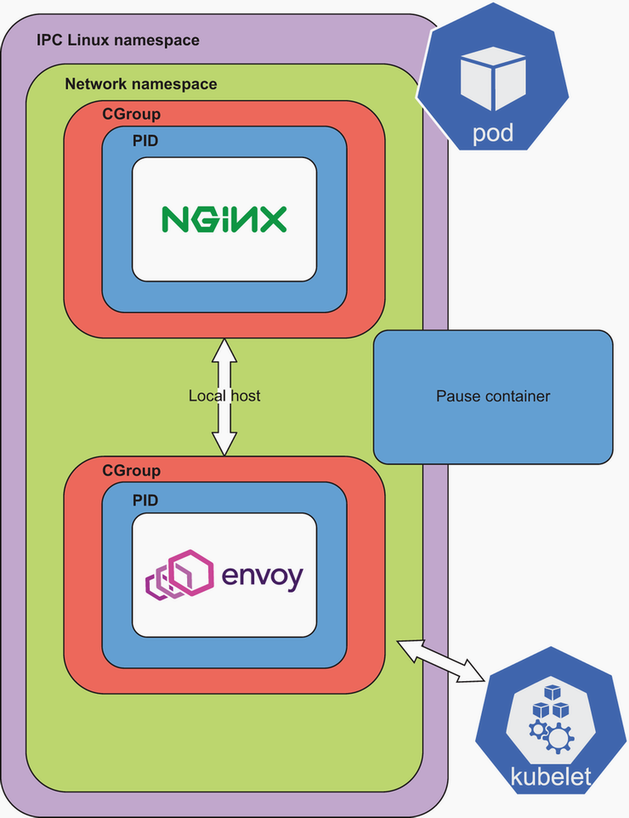
\includegraphics[width=0.7\textwidth]{capitulos/img/image4.png} % Cambia esto por el nombre de tu archivo de imagen
    \caption{El Pod como abstracción que encapsula uno o más contenedores (Figura 2.1).}
    \label{fig:pod_concept}
\end{figure}
% -----------------------------------------------------------

Muchos otros objetos de la API de Kubernetes utilizan Pods directamente o son objetos diseñados para darles soporte. Por ejemplo, un objeto de tipo \textit{Deployment} utiliza Pods, al igual que los \textit{StatefulSets} y los \textit{DaemonSets}. Varios controladores de alto nivel de Kubernetes se encargan de crear y gestionar el ciclo de vida de los Pods. Los controladores son componentes de \textit{software} que se ejecutan en el plano de control; entre los ejemplos de controladores integrados se encuentran el \textit{controller manager}, el \textit{cloud manager} y el \textit{scheduler}. 

Antes de profundizar en ello, hagamos una pequeña digresión analizando una aplicación web para luego vincularla nuevamente con Kubernetes, el Pod y el plano de control.

\subsubsection*{Nota}
\textit{Es posible que note que utilizamos el término ``plano de control'' (\textit{control plane}) para definir al grupo de nodos que ejecutan el controlador, el administrador de controladores y el programador. En ocasiones también se les denomina ``maestros'' (\textit{masters}), pero en este libro utilizaremos exclusivamente ``plano de control'' al referirnos a estos componentes.}

\subsection{Ejemplo de una aplicación web (An example web application)}

Para comprender la necesidad de existencia del Pod y cómo Kubernetes soporta las aplicaciones contenedorizadas, analizaremos el caso de la empresa de bebidas energéticas \textit{Zeus Zap}. Su sitio web de comercio electrónico consta de tres capas: interfaz de usuario (UI), capa intermedia (microservicios) y base de datos en el \textit{backend}. 

Un desglose de una sección de su infraestructura tecnológica (Figura 2.2) incluye:
\begin{itemize}
    \item Un \textit{frontend} en JavaScript servido por \textit{NGINX}.
    \item Dos capas de controladores web que son microservicios en \textit{Python} desarrollados con \textit{Django}.
    \item Una base de datos \textit{CockroachDB} en el \textit{backend} que escucha en el puerto 6379, respaldada por almacenamiento persistente.
\end{itemize}

En un entorno de producción tradicional basado únicamente en contenedores independientes, el inicio de la aplicación se ejecutaría mediante los siguientes comandos de Docker:

\begin{verbatim}
$ docker run -t -i ui -p 80:80
$ docker run -t -i miroservice-a -p 8080:8080
$ docker run -t -i miroservice-b -b 8081:8081
$ docker run -t -i cockroach:cockroach -p 6379:6379
\end{verbatim}

\subsubsection{Limitaciones del enfoque tradicional y nuevos requisitos}
Al poner en marcha estos servicios bajo este esquema, la compañía rápidamente se enfrenta a varios problemas de diseño y arquitectura de infraestructura:
\begin{enumerate}
    \item \textbf{Conflictos de puertos:} No es posible ejecutar múltiples copias del contenedor de la UI a menos que se coloque un balanceador de carga externo frente al puerto 80, ya que solo existe un puerto 80 disponible en la máquina host.
    \item \textbf{Rigidez de red:} No se puede migrar el contenedor de la base de datos (\textit{CockroachDB}) a otro servidor a menos que se modifique e inyecte dinámicamente la nueva dirección IP en la aplicación web (o se implemente un servidor DNS que se actualice dinámicamente con los movimientos del contenedor).
    \item \textbf{Restricciones de alta disponibilidad:} Cada instancia de la base de datos debe ejecutarse en un servidor físico diferente para garantizar una tolerancia a fallos real.
    \item \textbf{Persistencia y recuperación volátil:} Si una instancia de la base de datos falla, se requiere un mecanismo para mover sus datos a un nuevo nodo y reclamar el espacio de almacenamiento no utilizado en el host anterior.
\end{enumerate}

A raíz de esto, surgen requisitos fundamentales que una plataforma de orquestación de contenedores debe resolver:
\begin{itemize}
    \item \textbf{Red compartida:} Permitir que cientos de procesos compartan la red de manera inteligente sin generar conflictos al enlazarse a los mismos puertos.
    \item \textbf{Desacoplamiento de almacenamiento:} Migrar y separar los volúmenes de datos de los binarios de la aplicación, evitando ensuciar los discos locales de los servidores.
    \item \textbf{Optimización de recursos:} Maximizar el uso de la CPU y la memoria disponibles para reducir costos operativos.
\end{itemize}

\subsubsection*{Nota: El fenómeno del vecino ruidoso (\textit{Noisy Neighbor})}
\textit{Ejecutar múltiples procesos concurrentes en un mismo servidor suele provocar que las aplicaciones compitan de forma agresiva por recursos escasos (CPU, memoria). Un sistema de orquestación eficiente debe mitigar este comportamiento para asegurar un rendimiento predecible.}

Por lo tanto, gestionar aplicaciones contenedorizadas a gran o pequeña escala exige un mayor nivel de control en los siguientes aspectos:
\begin{itemize}
    \item \textbf{Planificación consciente del almacenamiento (\textit{Storage-aware scheduling}):} Capacidad de programar la ejecución de un proceso en estricta coordinación con la disponibilidad de sus datos.
    \item \textbf{Balanceo de carga consciente del servicio (\textit{Service-aware network load balancing}):} Redirigir el tráfico hacia las nuevas direcciones IP de forma transparente a medida que los contenedores migran de una máquina a otra.
\end{itemize}

% --- CÓDIGO PARA INSERTAR LA IMAGEN DE LA APLICACIÓN (Figura 2.2) ---
\begin{figure}[htbp]
    \centering
    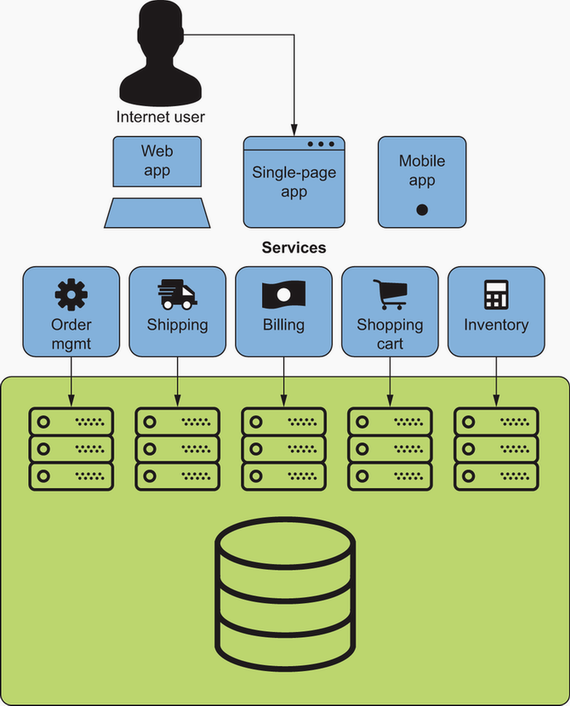
\includegraphics[width=0.85\textwidth]{capitulos/img/image5.png} % Cambia esto por el nombre de tu archivo de imagen
    \caption{Arquitectura de microservicios de Zeus Zap y sus desafíos de red y almacenamiento (Figura 2.2).}
    \label{fig:zeus_zap_architecture}
\end{figure}
% -------------------------------------------------------------------

Estas revelaciones tecnológicas coinciden con las mismas necesidades que dieron origen a las herramientas de orquestación y planificación distribuida de la década de 2000, tales como \textit{Borg} (el sistema interno de orquestación de contenedores de Google) y \textit{Mesos} (una aplicación de código abierto), ambos predecesores históricos de Kubernetes.

\subsection{Infraestructura para nuestra aplicación web (Infrastructure for our web application)}

Sin un \textit{software} de orquestación de contenedores como Kubernetes, las organizaciones requieren una gran cantidad de componentes independientes en su infraestructura. Para ejecutar una aplicación tradicional, se necesitan múltiples máquinas virtuales (VM) en la nube o servidores físicos, además de identificadores estables (como IPs estáticas o registros DNS) para localizar los servicios.

Las cargas de trabajo de los servidores varían significativamente según su propósito:
\begin{itemize}
    \item \textbf{Optimización de hardware:} Las bases de datos suelen requerir servidores con mucha memoria RAM y almacenamiento de baja latencia (como SSDs de alto rendimiento). Por el contrario, los microservicios pueden demandar más capacidad de cómputo (CPUs) pero menos memoria.
    \item \textbf{Almacenamiento diferenciado:} Las copias de seguridad o las aplicaciones que procesan datos en memoria y rara vez tocan el disco pueden utilizar un almacenamiento mucho más lento y económico.
    \item \textbf{Gestión de accesos y seguridad:} Los servidores de integración continua (como \textit{Jenkins} o \textit{CircleCI}) exigen un acceso completo de escritura a los servidores, mientras que los sistemas de monitoreo solo requieren acceso de lectura para recolectar métricas. A esto se le debe sumar la gestión de autenticación y autorización para el personal humano.
\end{itemize}

En resumen, una plataforma de despliegue propia exige aprovisionar de forma independiente: una plataforma base (VM o servidores físicos), balanceadores de carga, sistemas de descubrimiento de aplicaciones, soluciones de almacenamiento y sistemas de seguridad. 

Para sostener este ecosistema operativo, el equipo de DevOps se ve obligado a mantener (además de muchos otros subsistemas):
\begin{itemize}
    \item Sistemas de registro centralizado (\textit{logging}).
    \item Herramientas de monitoreo, alertas y métricas.
    \item Flujos de integración y entrega continua (CI/CD).
    \item Respaldos de seguridad (\textit{backups}).
    \item Gestión de secretos y credenciales.
\end{itemize}

A diferencia de estas plataformas caseras de entrega de aplicaciones, Kubernetes ofrece ventajas inmediatas de forma nativa (\textit{out of the box}), tales como rotación de registros, herramientas de inspección y gestión integrada de logs, lo que reduce drásticamente la sobrecarga operativa antes de enfrentarse a los verdaderos desafíos del negocio.

\subsection{Requisitos operacionales (Operational requirements)}

A diferencia de los minoristas tradicionales, la empresa de bebidas energéticas \textit{Zeus Zap} no experimenta un crecimiento estacional típico, sino que enfrenta picos masivos de demanda vinculados a su patrocinio de eventos de deportes electrónicos (\textit{e-sports}). Las campañas de marketing y las promociones en directo junto a \textit{streamers} generan uno de los patrones de tráfico más difíciles de gestionar para el equipo de DevOps: el \textbf{tráfico de ráfaga} (\textit{burst traffic}). 

Debido al impacto de las redes sociales durante estos eventos, la empresa está sumamente preocupada por las caídas del sistema, ya que los costos asociados al tiempo de inactividad (\textit{downtime}) son devastadores:

\begin{itemize}
    \item \textbf{Costo económico:} De acuerdo con un estudio de Gartner, el costo promedio de la inactividad de TI se estima en \$5,600 dólares por minuto. Una interrupción de apenas dos horas puede traducirse en una pérdida promedio de \$672,000 dólares.
    \item \textbf{Costo humano:} Los fallos constantes en la infraestructura desgastan al personal técnico. El agotamiento laboral (\textit{burnout}) de los empleados cuesta a las industrias estadounidenses entre \$125 y \$190 mil millones de dólares anuales.
\end{itemize}

Para mitigar esto, la mayoría de las empresas exigen altos niveles de disponibilidad y redundancia, tanto a nivel de \textit{software} como de hardware, además de mecanismos para revertir cambios (\textit{rollbacks}). Sin embargo, para mantener los presupuestos bajo control, estas mismas organizaciones necesitan reducir la infraestructura durante los períodos de menor demanda. 

Por lo tanto, la gestión de costos suele entrar en conflicto directo con los requisitos de disponibilidad del negocio. En resumen, una aplicación web moderna requiere equilibrar de manera eficiente cuatro pilares esenciales:
\begin{enumerate}
    \item \textbf{Escalabilidad:} Capacidad de responder a ráfagas imprevistas de tráfico.
    \item \textbf{Alta disponibilidad:} Redundancia para evitar puntos únicos de fallo.
    \item \textbf{Control de versiones:} Facilitar despliegues seguros y actualizaciones reversibles.
    \item \textbf{Gestión de costos:} Optimización y dimensionamiento elástico de los recursos.
\end{enumerate}

\subsection{El Pod como unidad de despliegue (The Pod as a deployment unit)}

A grandes rasgos, un \textbf{Pod} está compuesto por una o más imágenes OCI que se ejecutan como contenedores en un nodo de un clúster de Kubernetes. El nodo es una unidad de cómputo (un servidor) que ejecuta el agente \texttt{kubelet} y que, al igual que los demás componentes de la plataforma, se representa como un objeto de la API.

Desplegar un Pod de forma directa es tan sencillo como crear su manifiesto y enviarlo al clúster mediante la línea de comandos:

\begin{verbatim}
$ cat << EOF > pod.yaml
apiVersion: v1                              # 1. Versión de la API en el servidor
kind: Pod                                   # 2. Tipo de objeto de la API
metadata:
  name: busybox
spec:
  containers:
    - name: busybox
      image: mycontainerregistry.io/foo     # 3. Nombre de la imagen en el registro
EOF
$ kubectl create -f pod.yaml                # 4. Comando de ejecución de kubectl
\end{verbatim}

La herramienta \texttt{kubectl} actúa como la interfaz de línea de comandos principal para interactuar mediante peticiones REST con el servidor de la API de Kubernetes. Al arrancar el Pod, se puede verificar su ejecución dentro del espacio de nombres por defecto utilizando el comando \texttt{kubectl get po}.

\subsubsection{Abstracciones de alto nivel}
En la práctica, los Pods rara vez se despliegan de forma directa o aislada. En su lugar, el usuario define objetos de la API de nivel superior que se encargan de crear y gestionar el ciclo de vida de los Pods de forma automatizada:

\begin{itemize}
    \item \textbf{Deployments:} El objeto más utilizado en Kubernetes; es el estándar para desplegar aplicaciones sin estado (\textit{stateless}) como los microservicios.
    \item \textbf{Jobs:} Ejecutan Pods diseñados para realizar tareas por lotes (\textit{batch processes}) que finalizan tras completar su función.
    \item \textbf{StatefulSets:} Diseñados para alojar aplicaciones con estado (\textit{stateful}) como las bases de datos. Sus características principales incluyen:
    \begin{itemize}
        \item Nombramiento ordinal de Pods para garantizar identificadores de red únicos y estables.
        \item Almacenamiento persistente vinculado de forma estricta siempre al mismo Pod.
        \item Mecanismos ordenados para el arranque, escalado y actualización de las instancias.
    \end{itemize}
    \item \textbf{DaemonSets:} Se utilizan para garantizar que una copia de un Pod específico se ejecute como un ``agente'' en cada uno de los nodos del clúster (común para servicios del sistema como redes, almacenamiento o recolección de \textit{logs}).
\end{itemize}

\subsubsection*{Consejo práctico: Evitar la etiqueta \texttt{latest} en producción}
\textit{Los registros de contenedores permiten etiquetar imágenes con el tag \texttt{latest}. Se desaconseja totalmente su uso en entornos de producción, ya que este puntero no es inmutable y puede provocar fallos catastróficos al descargar inadvertidamente versiones de software no probadas. La mejor práctica exige utilizar siempre etiquetas con versiones específicas o, idealmente, el \textbf{SHA} (hash) de la imagen, el cual sí garantiza una inmutabilidad real.}

\subsubsection{El flujo de la aplicación Zeus Zap}
Para la aplicación web de \textit{Zeus Zap}, en lugar de depender de configuraciones locales que disparen comandos individuales de Docker (\texttt{docker run}) al iniciar un servidor, se utilizan abstracciones como \textit{Deployments} y \textit{StatefulSets}. Estos controladores de alto nivel generan objetos de réplica (\textit{ReplicaSets}), los cuales se encargan finalmente de instanciar y empaquetar los binarios y dependencias dentro de los Pods (Figura 2.3).

% --- CÓDIGO PARA INSERTAR LA IMAGEN DEL FLUJO DE PODS (Figura 2.3) ---
\begin{figure}[htbp]
    \centering
    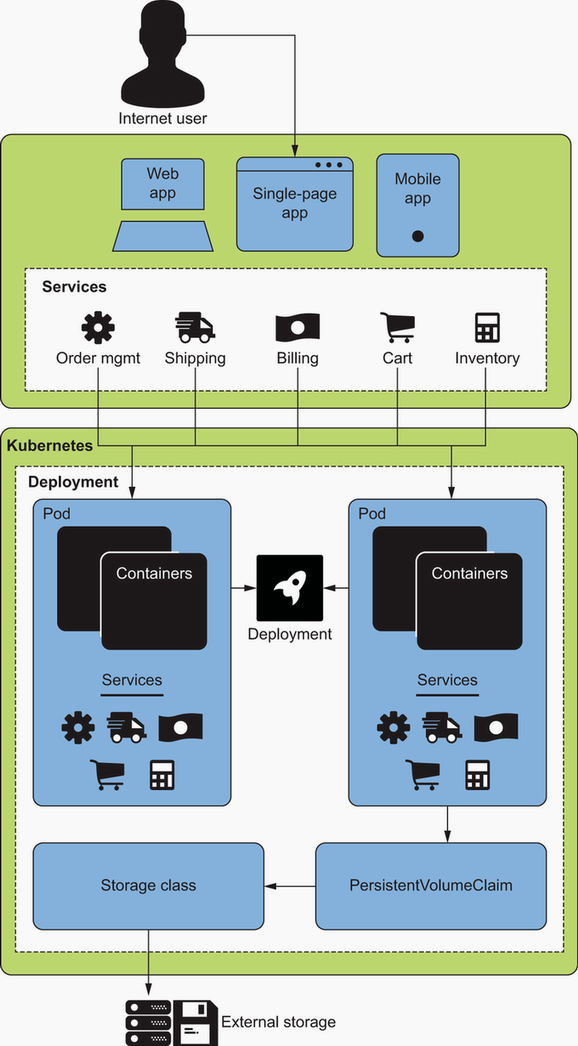
\includegraphics[width=0.85\textwidth]{capitulos/img/image6.png} % Cambia esto por el nombre de tu archivo de imagen
    \caption{Controladores de alto nivel (Deployments/StatefulSets) gestionando el ciclo de vida de los Pods de Zeus Zap (Figura 2.3).}
    \label{fig:zeus_zap_pods_flow}
\end{figure}
% ---------------------------------------------------------------------

\subsection{Espacios de nombres de Linux vs. Kubernetes (A bunch of Linux namespaces)}

Es fundamental no confundir los \textbf{Namespaces de Kubernetes} (aquellos creados con \texttt{kubectl create ns}) con los \textbf{namespaces de Linux}. Mientras que los primeros son abstracciones lógicas de la API para organizar recursos, los namespaces de Linux son una característica nativa del kernel que permite el aislamiento y la separación de procesos. 

A nivel elemental, un Pod es simplemente un conjunto de namespaces de Linux configurados de una forma específica. Un Pod comparte y encapsula los siguientes namespaces del kernel:
\begin{itemize}
    \item Uno o más namespaces de \textbf{PID} (identificadores de procesos).
    \item Un único namespace de \textbf{red} (\textit{networking}).
    \item Namespace de \textbf{IPC} (comunicación entre procesos).
    \item Namespace de \textbf{cgroup} (grupos de control para el límite de recursos).
    \item Namespace de \textbf{mnt} (puntos de montaje del sistema de archivos).
    \item Namespace de \textbf{user} (identificadores de usuario y grupo).
提供
\end{itemize}

Estos namespaces de Linux actúan como componentes del sistema de archivos del kernel que proveen la funcionalidad base para tomar una imagen y transformarla en un contenedor en ejecución.

\subsubsection{Relación con los requisitos de la aplicación}
¿Por qué es importante entender esto? Si volvemos a los requisitos operativos de la aplicación web de \textit{Zeus Zap}, la capacidad de escalar es vital. El Pod no solo nos otorga la facultad de desplegar contenedores, sino que permite escalar la infraestructura para manejar picos de tráfico. Para reducir costos y escalar verticalmente de manera eficiente, es imprescindible tener la capacidad de ajustar de forma aislada los límites de recursos de un contenedor (mediante el namespace de \textit{cgroup}).

Asimismo, para que los microservicios de la empresa se comuniquen de forma fiable con el servidor de \textit{CockroachDB}, se requiere un sistema definitivo de red y resolución de servicios. El Pod —y su base en los namespaces de Linux— proporciona el soporte para todas estas características. 

Dentro del namespace de red del Pod existe una pila de red virtualizada que se conecta directamente a un sistema de \textbf{Red Definida por Software (SDN)} que se extiende a lo largo de todo el clúster de Kubernetes. De este modo, la necesidad de escalar mediante el balanceo de carga entre múltiples Pods se ve totalmente respaldada por este \textit{framework} de red unificado.

\subsection{Kubernetes, la infraestructura y el Pod (Kubernetes, infrastructure, and the Pod)}

Dentro de Kubernetes, una unidad de potencia de cómputo (CPU y memoria) se representa mediante un objeto de la API denominado \textbf{Node} (Nodo). Un nodo es simplemente un servidor que ejecuta un conjunto de componentes definidos. Los requisitos esenciales de un nodo incluyen:

\begin{itemize}
    \item Un servidor (físico o virtual).
    \item Un sistema operativo instalado (con soporte para distribuciones de Linux o Windows).
    \item \textbf{systemd}: El administrador de sistema y servicios de Linux.
    \item \textbf{El kubelet}: El agente principal del nodo.
    \item \textbf{El entorno de ejecución de contenedores} (\textit{Container Runtime}, como Docker Engine, CRI-O o LXC).
    \item \textbf{kube-proxy}: El proxy de red que gestiona los servicios de Kubernetes.
    \item Un proveedor de \textbf{CNI} (\textit{Container Network Interface}).
\end{itemize}

Un nodo puede ejecutarse en plataformas tan diversas como una \textit{Raspberry Pi} o una máquina virtual en la nube. 

% --- CÓDIGO PARA INSERTAR LA IMAGEN DE LOS COMPONENTES DEL NODO (Figura 2.4) ---
\begin{figure}[htbp]
    \centering
    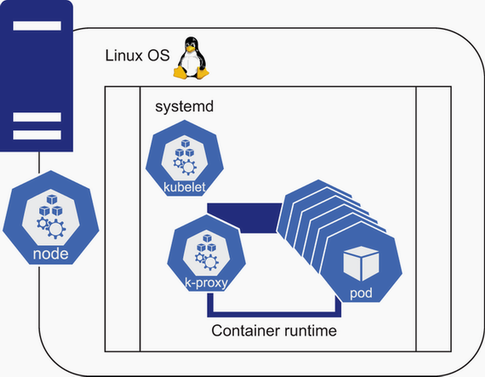
\includegraphics[width=0.85\textwidth]{capitulos/img/image7.png} % Cambia esto por el nombre de tu archivo de imagen
    \caption{Componentes internos de un nodo de Kubernetes ejecutándose sobre Linux (Figura 2.4).}
    \label{fig:linux_node_components}
\end{figure}
% -------------------------------------------------------------------------------

\subsubsection{El rol crítico del Kubelet}
El \texttt{kubelet} es un programa binario que se ejecuta como un agente en cada nodo y se comunica constantemente con el \textit{API server} a través de múltiples bucles de control (\textit{control loops}). Sin este componente, un nodo no puede programar tareas ni considerarse parte del clúster. Comprender el \texttt{kubelet} es clave para diagnosticar problemas de bajo nivel (por ejemplo, por qué un nodo no se une al clúster o por qué un Pod no se despliega). 

El \texttt{kubelet} garantiza lo siguiente:
\begin{itemize}
    \item Que cualquier Pod programado en su host se ejecute correctamente mediante la vigilancia continua del estado del clúster.
    \item Informar al \textit{API server} que el nodo está saludable a través de un mecanismo de latido (\textit{heartbeat}), el cual se gestiona en el espacio de nombres \texttt{kube-node-lease}.
    \item Recolectar la basura (\textit{garbage collection}) de los Pods cuando sea necesario, eliminando almacenamiento efímero o dispositivos de red huérfanos.
\end{itemize}

El \texttt{kubelet} no realiza el trabajo de aislamiento de forma directa; depende de una interfaz de tiempo de ejecución de contenedores (\textbf{CRI}) y de un proveedor de \textbf{CNI} para reconciliar el estado del nodo con los deseos del plano de control. Por ejemplo, si el plano de control decide desplegar un contenedor, el \texttt{kubelet} instruye al proveedor de CRI para que descargue la imagen del registro y asigne una dirección IP dentro del rango \texttt{podCIDR} del nodo.

\subsubsection{Servicios y el Proxy de Red (kube-proxy)}
El \textbf{Service} (Servicio) es otro objeto fundamental de la API. El componente binario \texttt{kube-proxy} se encarga de gestionar la creación y el mapeo de red de estos servicios en cada nodo. Los tipos principales de servicios son:

\begin{itemize}
    \item \textbf{ClusterIP:} Un servicio interno que balancea la carga entre los Pods dentro del clúster.
    \item \textbf{NodePort:} Abre un puerto estático en la IP de cada nodo para exponer y balancear la carga hacia los Pods externamente.
    \item \textbf{LoadBalancer:} Crea un balanceador de carga externo al clúster (generalmente integrado con el proveedor de la nube).
\end{itemize}

El \texttt{kube-proxy} facilita que cada nodo del clúster conozca la ubicación de cada servicio y cada Pod, soportando protocolos de red TCP, UDP y SCTP, así como el reenvío de tráfico.

\subsubsection*{Nota sobre redes en Kubernetes}
\textit{La conectividad de red se proporciona mediante una solución de software llamada proveedor de CNI. Actualmente, algunos proveedores avanzados de CNI están desarrollando arquitecturas de software que reemplazan por completo a \texttt{kube-proxy}, permitiendo gestionar el tráfico de los servicios de forma más eficiente sin necesidad de utilizar las reglas tradicionales de \texttt{iptables} de Linux.}

\subsection{El objeto Node de la API (The Node API object)}

Los nodos proporcionan el soporte físico o virtual para los Pods, mientras que el plano de control define el grupo de nodos encargados de ejecutar los controladores del sistema, el administrador de controladores y el programador. Para listar los nodos de un clúster, se utiliza el siguiente comando básico:

\begin{verbatim}
$ kubectl get no                                     # 1. Forma abreviada de 'kubectl get nodes'
NAME                STATUS    ROLES   AGE  VERSION
kind-control-plane  NotReady  master  25s  v1.17.0   # 2. Salida de un clúster local 'kind'
\end{verbatim}

Para inspeccionar detalladamente la estructura del objeto \texttt{Node} en la API, se puede solicitar su salida en formato YAML (\texttt{kubectl get no kind-control-plane -o yaml}). A continuación, se desglosa el manifiesto de la API dividido en sus secciones principales:

\subsubsection{Metadatos y Especificaciones (\texttt{metadata} y \texttt{spec})}
\begin{verbatim}
apiVersion: v1
kind: Node
metadata:
  annotations:
    kubeadm.alpha.kubernetes.io/cri-socket: /run/containerd/containerd.sock  # 1. Socket de CRI (containerd)
    node.alpha.kubernetes.io/ttl: "0"
    volumes.kubernetes.io/controller-managed-attach-detach: "true"
  creationTimestamp: "2020-09-20T14:51:57Z"
  labels:                                                                    # 2. Etiquetas estándar del nodo
    beta.kubernetes.io/arch: amd64
    beta.kubernetes.io/os: linux
    kubernetes.io/arch: amd64
    kubernetes.io/hostname: kind-control-plane
    kubernetes.io/os: linux
    node-role.kubernetes.io/master: ""
  name: kind-control-plane
spec:
  podCIDR: 10.244.0.0/24                                                     # 3. Rango IP asignado por el CNI
  podCIDRs:
  - 10.244.0.0/24
\end{verbatim}

\subsubsection{Estado y Condiciones del Nodo (\texttt{status})}
La sección \texttt{status} es actualizada continuamente por el \texttt{kubelet} hacia el \textit{API server} para reportar la capacidad del host y sus condiciones de salud:

\begin{verbatim}
status:
  addresses:
  - address: 172.17.0.2
    type: InternalIP
  - address: kind-control-plane
    type: Hostname
  allocatable:             # Recursos disponibles para asignar a los Pods
    cpu: "2"
    memory: 2039264Ki
    pods: "110"
  capacity:                # Capacidad total real del hardware
    cpu: "2"
    memory: 2039264Ki
    pods: "110"
  conditions:              # Presiones del sistema detectadas por el kubelet
  - reason: KubeletHasSufficientMemory
    status: "False"        # False indica que el nodo está saludable y sin presión de memoria
    type: MemoryPressure
  - reason: KubeletHasNoDiskPressure
    status: "False"
    type: DiskPressure
  - reason: KubeletHasSufficientPID
    status: "False"
    type: PIDPressure
  - reason: KubeletReady
    status: "True"         # True indica que el nodo está listo para recibir cargas de trabajo
    type: Ready
\end{verbatim}

\subsubsection{Imágenes e Información del Sistema (\texttt{images} y \texttt{nodeInfo})}
El nodo almacena un registro de todas las imágenes de contenedores que se encuentran descargadas en su almacenamiento local, incluyendo los componentes centrales del propio Kubernetes:

\begin{verbatim}
  images:
  - names: ["k8s.gcr.io/etcd:3.4.3-0"]                # Base de datos del clúster
    sizeBytes: 289997247
  - names: ["k8s.gcr.io/kube-apiserver:v1.17.0"]      # Servidor de la API
    sizeBytes: 144347953
  - names: ["k8s.gcr.io/kube-proxy:v1.17.0"]          # Proxy de red de servicios
    sizeBytes: 132100734
  - names: ["docker.io/kindest/kindnetd:0.5.4"]       # Proveedor de red (CNI)
    sizeBytes: 113207016
  nodeInfo:                                           # Versiones del entorno y del SO
    containerRuntimeVersion: containerd://1.3.2
    kernelVersion: 4.19.76-linuxkit
    kubeletVersion: v1.17.0
    operatingSystem: linux
    osImage: Ubuntu 19.10
\end{verbatim}

---

\subsection{Controladores y bucles de control (Controllers and control loops)}

El término ``control'' está muy presente en Kubernetes. El sistema está compuesto por múltiples binarios ejecutables llamados \textbf{controladores} (como el \texttt{kubelet}, \texttt{kube-proxy} o el \texttt{scheduler}). Estos controladores se programan bajo un patrón de diseño de ingeniería de \textit{software} conocido como \textbf{bucles de control} (\textit{control loops}).

A grandes rasgos, Kubernetes actúa como una máquina de reconciliación de estados infinitamente activa, operando de manera similar a un termostato de aire acondicionado: mide constantemente el estado actual del sistema, lo compara con el estado deseado (definido por el usuario en los archivos YAML) y realiza las acciones necesarias para corregir cualquier desviación. 

En lugar de regular la temperatura, los bucles de control de Kubernetes regulan aspectos críticos de los sistemas distribuidos:
\begin{itemize}
    \item Vincular y montar de forma dinámica el almacenamiento persistente a los procesos.
    \item Crear contenedores en ejecución y escalar el número de réplicas bajo demanda.
    \item Terminar y migrar contenedores hacia nodos sanos si se detectan fallos de salud.
    \item Configurar rutas IP hacia puertos específicos.
    \item Actualizar dinámicamente los \textit{endpoints} de los balanceadores de carga.
\end{itemize}

\subsubsection{Reconciliación de los requisitos previos}
Vinculando todo lo aprendido hasta ahora: los Pods nos proveen el instrumento para desplegar imágenes; el \texttt{kubelet} gestiona localmente su ciclo de vida dentro del nodo; los objetos \texttt{Service} y el balanceo interno son administrados por el \texttt{kube-proxy}; y un sistema DNS (como \texttt{CoreDNS}) permite el descubrimiento entre aplicaciones para que, por ejemplo, el microservicio de \textit{Zeus Zap} localice y consuma la base de datos \textit{CockroachDB}. Para el almacenamiento persistente, la combinación del namespace de Linux \texttt{mnt} junto con el \texttt{kubelet} permite montar dinámicamente un disco duro al Pod durante su creación.

Sin embargo, aún faltan resolver preguntas clave de arquitectura global: ¿Qué ocurre si un nodo entero muere? ¿Cómo se decide inicialmente a qué nodo específico debe asignarse un Pod? Para dar respuesta a estas necesidades de orquestación distribuida, entra en juego el \textbf{plano de control} (\textit{control plane}).

\subsection{Nuestra aplicación web y el plano de control (Our web application and the control plane)}

Una vez establecidos los Pods y los nodos, el siguiente paso lógico es resolver los requisitos arquitectónicos complejos, tales como la \textbf{alta disponibilidad} (\textit{HA - High Availability}). La alta disponibilidad no consiste simplemente en un mecanismo de conmutación por error (\textit{failover}), sino en el cumplimiento estricto de un Acuerdo de Nivel de Servicio (\textit{SLA - Service-Level Agreement}). 

La disponibilidad del sistema se mide habitualmente mediante el ``número de nueves'' de tiempo de actividad (\textit{uptime}):
\begin{itemize}
    \item \textbf{Cuatro nueves (99.99\%):} Permiten un máximo de 52 minutos y 36 segundos de inactividad al año.
    \item \textbf{Cinco nueves (99.999\%):} Reducen el margen a tan solo 5 minutos y 15 segundos de inactividad anual (lo que equivale a apenas 26.25 segundos al mes).
\end{itemize}

Alcanzar un nivel de disponibilidad de cinco nueves significa que el sistema debe ser capaz de recuperarse de forma casi instantánea. Junto a la alta disponibilidad, coexisten otros objetivos operacionales críticos que Kubernetes ayuda a gestionar bajo la misma plataforma:
\begin{enumerate}
    \item Escalabilidad elástica e inmediata.
    \item Reducción y optimización de costos de infraestructura.
    \item Control de versiones de los contenedores para despliegues y regresiones (\textit{rollbacks}).
    \item Seguridad integral, tanto para los usuarios como en la comunicación entre aplicaciones.
\end{enumerate}

\subsubsection*{Nota sobre el diseño de aplicaciones}
\textit{Si bien Kubernetes proporciona de forma nativa todas estas capacidades de resiliencia y escalado, las aplicaciones deben estar diseñadas para alinearse y soportar los patrones arquitectónicos nativos de la nube bajo los cuales opera la plataforma.}

El punto de partida de todo este engranaje es el aprovisionamiento automatizado de los Pods. A partir de ahí, el plano de control asume la responsabilidad de actuar como el cerebro del clúster, coordinando la tolerancia a fallos y la distribución eficiente de las cargas de trabajo para maximizar el ahorro económico.

% --- CÓDIGO PARA INSERTAR LA IMAGEN DEL PLANO DE CONTROL (Figura 2.5) ---
\begin{figure}[htbp]
    \centering
    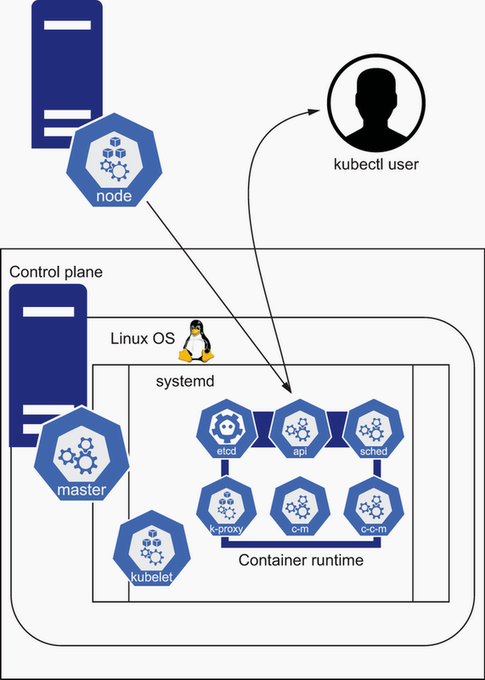
\includegraphics[width=0.85\textwidth]{capitulos/img/image8.png} % Cambia esto por el nombre de tu archivo de imagen
    \caption{Componentes principales que integran el plano de control (Control Plane) de Kubernetes (Figura 2.5).}
    \label{fig:kubernetes_control_plane}
\end{figure}
% -----------------------------------------------------------------------

\subsection{Creación de una aplicación web con kubectl (Creating a web application with kubectl)}

Para comprender cómo el plano de control gestiona y facilita operaciones complejas —como el escalado automático y la tolerancia a fallos—, analizaremos lo que sucede internamente al ejecutar el comando básico: \texttt{kubectl apply -f deployment.yaml}. 

El siguiente manifiesto representa la definición YAML estándar para este objeto de tipo \textit{Deployment}:

\begin{verbatim}
apiVersion: apps/v1
kind: Deployment
metadata:
  name: nginx
spec:
  replicas: 3                                # Número deseado de copias concurrentes
  selector:
    matchLabels:
      app: nginx
  template:                                  # Plantilla para la creación de los Pods
    metadata:
      labels:
        app: nginx
    spec:
      containers:
      - name: nginx
        image: nginx:1.7.9                   # Imagen OCI y versión específica
        ports:
        - containerPort: 80                  # Puerto expuesto dentro del contenedor
\end{verbatim}

En el momento exacto en que se ejecuta el comando \texttt{kubectl apply}, la herramienta de línea de comandos procesa el archivo y se comunica directamente con el primer componente y la puerta de entrada principal del plano de control: el **servidor de la API** (\textit{API server}).

\subsection{El servidor de la API de Kubernetes: \texttt{kube-apiserver}}

El servidor de la API de Kubernetes, \texttt{kube-apiserver}, es un servidor REST basado en HTTP que expone todos los objetos de la API de un clúster, desde Pods y nodos hasta componentes como el \textit{Horizontal Pod Autoscaler}. Este componente valida las peticiones y proporciona la interfaz web necesaria para realizar operaciones CRUD sobre el estado compartido del clúster. 

En entornos de producción, el plano de control suele ofrecer una infraestructura robusta para el \textit{API server}. Esto implica ejecutarlo de manera redundante en cada nodo del plano de control o delegarlo en un servicio de nube gestionado que garantice su alta disponibilidad. En la práctica, el acceso a la API se canaliza a través de un balanceador de carga de la nube o un proxy como \textit{HAProxy}.

Todos los componentes del plano de control se comunican exclusivamente a través del \textit{API server}:
\begin{itemize}
    \item Cuando un nodo arranca, su agente \texttt{kubelet} se registra en el clúster comunicándose con la API.
    \item Todos los controladores del plano de control ejecutan un bucle de control con funcionalidad de vigilancia (\textit{watch}) para monitorizar en tiempo real cualquier cambio en los objetos de la API.
\end{itemize}

\subsubsection{Persistencia y Seguridad}
El \textit{API server} es el único componente del plano de control autorizado para comunicarse directamente con \textbf{etcd}, la base de datos de Kubernetes. Aunque en el pasado algunos componentes de red (CNI) accedían a ella de forma directa, la arquitectura actual centraliza todo a través de la API, proporcionando una interfaz con estado para cualquier modificación del clúster. Por este motivo, proteger los puntos de acceso HTTPS del \textit{API server} es un pilar crítico en la seguridad del sistema.

Al operar en un plano de control de alta disponibilidad, todas las instancias del \textit{API server} están activas y reciben tráfico simultáneamente, ya que se trata de un componente principalmente sin estado (\textit{stateless}). 

Para evitar accesos no autorizados, el servidor de la API integra controladores de admisión (\textit{admission controllers}) encargados de validar la \textbf{autenticación} y la \textbf{autorización} de cada cliente. Es común integrar sistemas externos de identidad mediante el uso de \textit{webhooks} (APIs HTTP PUSH para llamadas de retorno o \textit{callbacks}).

Una vez que la llamada de \texttt{kubectl} es correctamente autenticada y autorizada, el \textit{API server} persiste el nuevo objeto \textit{Deployment} en \texttt{etcd}. El siguiente paso en el flujo del plano de control es activar el programador (\textit{scheduler}) para asignarle un hogar físico a los nuevos Pods en algún nodo del clúster.

\subsection{El programador de Kubernetes: \texttt{kube-scheduler}}

La planificación distribuda de procesos es una tarea compleja. El programador de Kubernetes, \texttt{kube-scheduler}, proporciona una implementación limpia y directa para asignar recursos dentro del clúster, evaluando múltiples factores antes de decidir en qué nodo debe ejecutarse un Pod:

\begin{itemize}
    \item \textbf{Recursos de hardware:} Capacidad disponible de CPU y memoria en cada nodo del clúster.
    \item \textbf{Restricciones de políticas:} Reglas de cumplimiento y cuotas establecidas para la programación.
    \item \textbf{Afinidad y antiafinidad de Pods (\textit{Pod affinity / anti-affinity}):} Las reglas de afinidad atraen magnéticamente a los Pods hacia nodos específicos que cumplen ciertas características, mientras que las de antiafinidad los repelen para evitar, por ejemplo, que dos réplicas de la misma aplicación crítica compartan el mismo host físico.
    \item \textbf{Tolerancias y rechazos (\textit{Taints and tolerations}):} Los \textit{taints} permiten a un nodo repeler activamente un conjunto de Pods a menos que estos cuenten con una tolerancia específica, ayudando al programador a delimitar qué cargas de trabajo no deben mezclarse.
\end{itemize}

Retomando el ejemplo de la empresa \textit{Zeus Zap}, el manifiesto define tres réplicas para el Pod. Estas copias aseguran tanto la tolerancia a fallos como la capacidad de escalar; es el \texttt{kube-scheduler} el encargado de determinar de forma óptima sobre qué nodo o nodos específicos se distribuirán dichas réplicas.

\subsubsection{El ciclo de vida del Pod y aislamiento del plano de control}
Una vez que el \texttt{kube-scheduler} toma la decisión y actualiza el manifiesto del Pod inyectándole el campo \texttt{NodeName}, el \texttt{kubelet} de ese nodo específico toma el control del ciclo de vida del Pod y procede a desplegarlo localmente, actuando como un ``mini-programador'' del host.

El plano de control se encuentra completamente aislado y desacoplado de los nodos de trabajo (\textit{worker nodes}) que ejecutan las aplicaciones. Esto tiene implicaciones críticas de resiliencia:
\begin{itemize}
    \item \textbf{Tolerancia a fallos del plano de control:} Si ocurre una caída total del plano de control, la aplicación de \textit{Zeus Zap} no perderá información ni se interrumpirá. El sitio web seguirá activo y procesando tráfico de forma normal en los nodos de trabajo.
    \item \textbf{Limitaciones temporales:} Durante la caída del plano de control, simplemente se congela el estado del clúster: no se pueden desplegar nuevas aplicaciones ni realizar cambios de configuración, pero la infraestructura existente se mantiene intacta.
\end{itemize}

En caso de que las aplicaciones requieran el uso de un disco persistente, el almacenamiento continuará operando de manera independiente. Si un nodo de trabajo llegase a fallar de forma simultánea a una interrupción del plano de control, en cuanto este último vuelva a estar en línea, los controladores automatizados de Kubernetes se encargarán de realizar una migración segura tanto de los datos persistentes como de la aplicación hacia un nuevo nodo sano.

\subsection{Controladores de infraestructura y el patrón Operator (Infrastructure controllers)}

Ciertas aplicaciones con estado (\textit{stateful}), como la base de datos distribuida \textit{CockroachDB}, presentan requisitos operacionales complejos. Para gestionarlas de forma nativa en Kubernetes, se utiliza el patrón **Operator** (Operador), el cual se ha convertido en el estándar para desplegar componentes avanzados, reemplazando el uso de manifiestos YAML planos.

El siguiente ejemplo ilustra la instalación del Operador para \textit{CockroachDB}:
\begin{verbatim}
# 1. Instala las Definiciones de Recursos Personalizados (CRDs) del Operador
$ kubectl apply -f https://raw.githubusercontent.com/cockroachdb/cockroach-operator/master/install/crds.yaml

# 2. Instala el binario del Operador en el espacio de nombres por defecto
$ kubectl apply -f https://raw.githubusercontent.com/cockroachdb/cockroach-operator/master/install/operator.yaml
\end{verbatim}

\subsubsection{Definiciones de Recursos Personalizados (CRDs)}
Las **Custom Resource Definitions (CRDs)** son objetos de la API que permiten definir e introducir nuevos objetos personalizados dentro del propio servidor de la API de Kubernetes. Una vez aplicado el CRD, el clúster es capaz de entender y gestionar un nuevo tipo de recurso.

Tras descargar el archivo de ejemplo del operador (\texttt{curl -LO ...}), se puede desplegar un clúster de base de datos utilizando este recurso personalizado:

\begin{verbatim}
apiVersion: crdb.cockroachlabs.com/v1alpha1
kind: CrdbCluster
metadata:
  name: cockroachdb
spec:
  dataStore:
    pvc:
      spec:
        accessModes: [- ReadWriteOnce]
        resources:
          requests: {storage: "60Gi"}
        volumeMode: Filesystem
  resources:
    requests: {cpu: "2", memory: "8Gi"}
    limits: {cpu: "2", memory: "8Gi"}
  tlsEnabled: true
  image:
    name: cockroachdb/cockroach:v21.1.5     # 1. Contenedor de la base de datos
  nodes: 3
  additionalLabels:
    crdb: is-cool
\end{verbatim}

A partir de este bloque, el Operador se encarga de automatizar la creación de cientos de líneas de configuración subyacente: claves TLS almacenadas en \textit{Secrets}, un \textit{StatefulSet}, almacenamiento persistente (\textit{PersistentVolumeClaims}), servicios de red y presupuestos de disrupción de Pods (\textit{PDB}).

---

\subsection{El Administrador de Controladores: KCM y la evolución hacia el CCM}

Para dar vida a abstracciones como el almacenamiento persistente (\texttt{PersistentVolume} y \texttt{PersistentVolumeClaim}), Kubernetes se apoya en el **Kubernetes Controller Manager (KCM)** y el **Cloud Controller Manager (CCM)**. 

El KCM es un binario único que ejecuta múltiples bucles de control de forma simultánea. Históricamente, el KCM albergaba todo el código necesario para interactuar con los diferentes proveedores de infraestructura (GKE, AWS, vSphere, etc.). Sin embargo, la inclusión de código específico de cada proveedor dentro del repositorio principal de Kubernetes (\textit{kubernetes/kubernetes} o \textit{kk}) volvió el código fuente difícil de mantener.

\subsubsection{El nacimiento del Cloud Controller Manager (CCM)}
Para desacoplar a Kubernetes de tecnologías propietarias y hacerlo completamente agnóstico de la nube, el equipo de desarrollo (bajo la CNCF) introdujo el **CCM**. El CCM extrae la lógica específica de los proveedores de nube hacia repositorios independientes mantenidos por terceros (como DigitalOcean, AWS, etc.), permitiendo que estos avancen a mayor velocidad sin modificar el núcleo de Kubernetes.

Cuando el clúster se ejecuta en una nube pública o privada, el CCM intercepta las peticiones y ejecuta las llamadas necesarias hacia las APIs del proveedor a través de cuatro controladores principales:
\begin{itemize}
    \item \textbf{Node controller:} Sincroniza y valida el estado de los nodos con la infraestructura de la nube.
    \item \textbf{Route controller:} Configura las rutas de red y pasarelas en la infraestructura subyacente.
    \item \textbf{Service controller:} Gestiona la creación, actualización y eliminación de los balanceadores de carga de la nube.
    \item \textbf{Volume controller:} Orquesta la creación, el enganche (\textit{attach}) y el montaje de volúmenes de almacenamiento en la nube.
\end{itemize}

Esta modularidad se complementa con otras interfaces estandarizadas y neutrales dentro de la arquitectura de Kubernetes:
\begin{itemize}
    \item \textbf{CNI (Container Networking Interface):} Provee y asigna direcciones IP a los Pods.
    \item \textbf{CRI (Container Runtime Interface):} Permite conectar diferentes motores de ejecución de contenedores.
    \item \textbf{CSI (Container Storage Interface):} Permite a los proveedores de almacenamiento añadir soporte para nuevos tipos de discos sin alterar el código base del sistema.
\end{itemize}

\subsubsection{Flujo de aprovisionamiento de recursos}
Volviendo al caso de uso de \textit{Zeus Zap}, cuando el Operador solicita el despliegue de las réplicas de la base de datos, ocurre lo siguiente:
\begin{enumerate}
    \item El \texttt{kube-scheduler} asigna el Pod a un nodo específico.
    \item El KCM (o CCM) detecta la solicitud de almacenamiento persistente, interactúa con la API de la infraestructura para aprovisionar el disco y lo monta en el servidor host.
    \item El agente \texttt{kubelet} levanta el Pod y, utilizando el namespace de Linux \texttt{mnt}, conecta de forma segura dicho almacenamiento dentro del contenedor.
\end{enumerate}

Para exponer el sitio web público mediante un balanceador de carga externo, el usuario simplemente define un objeto de tipo \texttt{Service} configurado como \texttt{type: LoadBalancer}:

\begin{verbatim}
apiVersion: v1
kind: Service
metadata:
  name: example-service
spec:
  selector:
    app: example
  ports:
    - port: 8765
      targetPort: 9376
  type: LoadBalancer                         # Solicita un balanceador externo
\end{verbatim}

El bucle de vigilancia (\textit{watch loop}) del CCM detecta esta configuración, aprovisiona una dirección IP pública mediante las APIs de la nube y la vincula a los nodos del clúster. Finalmente, cuando el tráfico de los usuarios llega a los nodos del hardware externo, la red interna administrada por el proveedor de **CNI** se encarga de enrutar el paquete de forma transparente hasta el Pod correcto.


\subsection{Escalado, alta disponibilidad y gestión de fallos (Scaling, HA, and the control plane)}

El escalado elástico de las aplicaciones es el mecanismo subyacente que permite la alta disponibilidad (\textit{HA}) en la nube y, de forma más optimizada, en Kubernetes. Ante picos de demanda o fallos en la infraestructura, el sistema necesita instanciar más Pods o redesplegarlos en nodos sanos para mantener el nivel de servicio. 

El comando \texttt{kubectl scale} permite incrementar o disminuir de forma inmediata el número de Pods en ejecución, actuando directamente sobre controladores como \textit{ReplicaSets} o \textit{StatefulSets}:

\begin{verbatim}
$ kubectl scale --replicas 300 deployment zeus-front-end-ui
\end{verbatim}

% --- BLOQUE DE LA IMAGEN (FIGURA 2.6) ---
\begin{figure}[htbp]
    \centering
    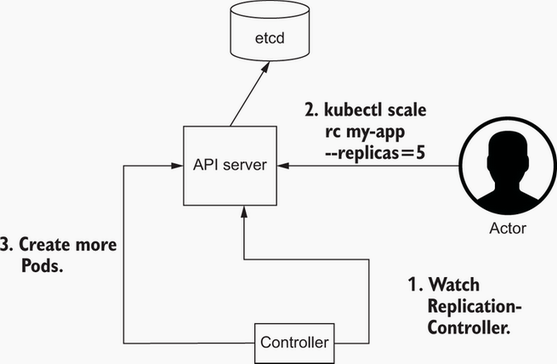
\includegraphics[width=0.9\textwidth]{capitulos/img/image9.png} % Reemplaza por el nombre real de tu archivo de imagen
    \caption{Secuencia típica y flujo de comunicación en el plano de control al ejecutar el comando \texttt{kubectl scale} (Figura 2.6).}
    \label{fig:kubernetes_scale_sequence}
\end{figure}
% ----------------------------------------

\subsubsection*{Nota sobre los DaemonSets}
\textit{Este comando de escalado no aplica a los objetos de tipo \textit{DaemonSet}. Por definición, un \textit{DaemonSet} ejecuta exactamente un Pod en cada nodo del clúster; por lo tanto, su escala está determinada estrictamente por el número de nodos físicos o virtuales que componen la infraestructura.}

En el escenario de \textit{Zeus Zap}, el comando anterior ajusta la cantidad de Pods que respaldan el \textit{frontend} de la UI, siguiendo el mismo flujo de comunicación entre el \textit{scheduler}, el KCM y el \texttt{kubelet}.

\subsubsection{Niveles de tolerancia a fallos y resiliencia}
Los fallos en producción son inevitables. Kubernetes clasifica y gestiona las acciones de recuperación ante incidentes en tres niveles operativos distintos:

\begin{enumerate}
    \item \textbf{Cortes a nivel de Pod:} El \texttt{kubelet} es el guardián del ciclo de vida del Pod en el host. Si el proceso del contenedor se detiene o si falla una prueba de vida (\textit{liveness probe}) definida por el usuario, el \texttt{kubelet} inicia un bucle de control para reiniciar automáticamente el Pod dañado.
    \item \textbf{Cortes a nivel de Nodo:} El \texttt{kubelet} envía constantemente una señal de latido (\textit{heartbeat}) al \textit{API server} a través del espacio de nombres \texttt{kube-node-lease}. Si un nodo deja de enviar este latido debido a un fallo de red o de hardware, el KCM cambia su estado a fuera de línea (\textit{offline}). Inmediatamente, se detiene la programación de nuevas cargas en él, y los Pods que residían allí se marcan para eliminación y se reprograman de forma automática en nodos sanos. Este comportamiento se puede emular manualmente utilizando los comandos \texttt{kubectl cordon} (marcar como no programable) y \texttt{kubectl drain} (evacuar el nodo).
    \item \textbf{Actualizaciones de software sin interrupciones:} Kubernetes está diseñado para realizar actualizaciones de la plataforma o de las versiones de las aplicaciones sin tiempo de inactividad (\textit{zero-downtime}). 
\end{enumerate}

\subsubsection*{Condición crítica: Durabilidad de la aplicación}
\textit{Para evitar la pérdida de datos durante los despliegues o fallos, el software que se ejecuta sobre Kubernetes debe ser resiliente y soportar un apagado e inicio gradual (\textit{graceful shutdown and startup}). Si una instancia se destruye a mitad de una transacción, la lógica de la aplicación debe ser capaz de reintentar dicha transacción en otra réplica o reanudarla de forma segura al reiniciarse.}

Actualizar la versión de un \textit{Deployment} es tan sencillo como modificar la etiqueta de la imagen en el archivo YAML. En el día a día, esto se realiza mediante tres comandos principales de la API:
\begin{itemize}
    \item \texttt{kubectl edit:} Abre el manifiesto del objeto directamente en un editor de texto de la terminal local para realizar cambios en caliente.
    \item \texttt{kubectl apply:} Toma un archivo de configuración local, contrasta las diferencias y reemplaza automáticamente el objeto modificado en el clúster.
    \item \texttt{kubectl patch:} Permite aplicar un pequeño fragmento de código (parche) para actualizar atributos muy específicos de un objeto sin necesidad de reescribir todo el archivo.
\end{itemize}


\subsection{Escalado automático (Autoscaling)}

Escalar los despliegues de forma manual es una excelente opción para gestionar cambios previstos, pero resulta inviable ante un incremento repentino de tráfico, como recibir 10,000 peticiones web nuevas por minuto. Para resolver este escenario, Kubernetes ofrece mecanismos de escalado automático (\textit{autoscaling}) que pueden configurarse en tres dimensiones distintas:

\begin{itemize}
    \item \textbf{Incrementar el número de Pods (Escalado Horizontal):} Gestionado por el objeto de la API \texttt{HorizontalPodAutoscaler} (HPA), el cual duplica o multiplica las instancias de los Pods según la demanda de tráfico o uso de CPU.
    \item \textbf{Asignar más recursos a los Pods existentes (Escalado Vertical):} Gestionado por el \texttt{VerticalPodAutoscaler} (VPA), el cual incrementa dinámicamente los límites de CPU y memoria de los Pods en ejecución.
    \item \textbf{Añadir más nodos al clúster (Escalado de Infraestructura):} Gestionado por el \texttt{Cluster Autoscaler}, el cual aprovisiona automáticamente nuevos servidores (nodos) cuando los recursos globales del clúster se agotan y los Pods no encuentran espacio para ejecutarse.
\end{itemize}

\subsubsection*{Nota sobre plataformas locales (\textit{Bare Metal})}
\textit{Dependiendo de la arquitectura de la infraestructura, los componentes de escalado automático (especialmente el \textit{Cluster Autoscaler}) podrían no estar disponibles de forma nativa en entornos que utilicen servidores físicos propios (\textit{bare metal}), requiriendo integraciones a medida con las APIs de virtualización locales.}

\subsection{Gestión de costos y densidad de Pods (Cost management)}

Cuando un clúster escala automáticamente (\textit{autoscaling}), añade nuevos nodos a la infraestructura, lo que incrementa de forma directa los costos de facturación en la nube. Aunque disponer de más nodos permite que las aplicaciones tengan más réplicas y soporten una mayor carga de trabajo, la optimización financiera exige buscar soluciones de ahorro. Aquí es donde entra en juego el concepto de **densidad de Pods** (\textit{Pod density}), que consiste en empaquetar de forma densa y eficiente los Pods dentro de los nodos existentes.

Dado que los Pods son la unidad básica de cómputo y los nodos (físicos o virtuales) representan el costo real del servidor, cuantos más Pods compartan un mismo nodo, menor será el gasto en servidores adicionales. Kubernetes permite alcanzar una alta densidad mediante el sobreaprovisionamiento de los hosts controlando los siguientes pasos esenciales:

\begin{enumerate}
    \item \textbf{Dimensionar y perfilar las aplicaciones:} Es imprescindible probar y perfilar cada aplicación para conocer su consumo real de CPU y memoria. Una vez analizadas, se deben configurar adecuadamente las restricciones y límites de recursos (\textit{resource limits}) en sus manifiestos de Kubernetes.
    \item \textbf{Seleccionar el tamaño óptimo de los nodos:} Elegir tamaños de máquinas virtuales o servidores \textit{bare metal} con capacidades de hardware heterogéneas permite consolidar múltiples aplicaciones en un mismo host. A pesar de buscar la máxima densidad, se debe mantener un número mínimo de nodos que garantice la alta disponibilidad exigida por los acuerdos de nivel de servicio (\textit{SLA}).
    \item \textbf{Agrupar aplicaciones estratégicamente:} Consiste en rellenar los huecos de recursos combinando cargas de trabajo grandes con aplicaciones más pequeñas (análogo a llenar un frasco con canicas y luego verter arena en los espacios vacíos). Las restricciones de asignación como los \textit{taints} (rechazos) y \textit{tolerations} (tolerancias) permiten a los operadores controlar este empaquetado.
\end{enumerate}

\subsubsection{Mitigación del vecino ruidoso (\textit{Noisy Neighbors}) y apagado programado}
El empaquetado denso introduce el riesgo del fenómeno del \textbf{vecino ruidoso}, donde aplicaciones con picos agresivos de consumo compiten por recursos escasos afectando a los contenedores adyacentes. Para mitigar esto, Kubernetes permite distribuir estas aplicaciones problemáticas de manera uniforme a lo largo del clúster utilizando reglas de **afinidad y antiafinidad de Pods** (\textit{Pod affinity / anti-affinity}). 



Adicionalmente, se pueden lograr mayores ahorros económicos combinando el escalado automático con el uso de máquinas virtuales efímeras en la nube (\textit{Spot/Ephemeral VMs}), o implementando políticas de apagado programado. Si los clústeres dedicados a entornos de Desarrollo o Control de Calidad (\textit{QA}) no se utilizan durante los fines de semana, la mejor estrategia de optimización consiste simplemente en reducir a cero el conteo de los nodos de trabajo (\textit{worker nodes}) y volver a escalarlos al inicio de la jornada laboral.

\subsection{Resumen del capítulo (Summary)}

\begin{itemize}
    \item \textbf{El Pod como unidad fundamental:} El Pod es el objeto básico de la API de Kubernetes que utiliza los \textit{namespaces} de Linux para crear un entorno aislado en el que se ejecutan uno o más contenedores de forma conjunta.
    \item \textbf{Patrones de diseño de la API:} Kubernetes fue diseñado para gestionar los Pods a través de diferentes patrones de abstracción de nivel superior, los cuales se representan como objetos de la API (tales como \textit{Deployments}, \textit{StatefulSets}, \textit{DaemonSets} y \textit{Jobs}).
    \item \textbf{Controladores y gestión del ciclo de vida:} Los controladores son los componentes de \textit{software} encargados de crear, vigilar y mantener el ciclo de vida de los Pods. Entre los más críticos se encuentran el \texttt{kubelet} (agente del nodo), el \textit{Cloud Controller Manager} (CCM) y el \texttt{kube-scheduler} (programador).
    \item \textbf{El plano de control como el cerebro del sistema:} A través de sus bucles de control distribuidos, el plano de control centraliza y automatiza tareas complejas de los sistemas distribuidos: vincula almacenamiento persistente a los procesos, escala el número de contenedores, destruye y migra instancias cuando están insalubres, configura rutas IP hacia los puertos y actualiza dinámicamente los \textit{endpoints} de los balanceadores de carga.
    \item \textbf{El Servidor de la API como punto de entrada único:} El componente \texttt{kube-apiserver} actúa como un servidor REST que valida y proporciona la interfaz web para realizar operaciones CRUD sobre el estado compartido del clúster. En entornos de producción, se ejecuta de forma redundante en todos los nodos del plano de control para garantizar una arquitectura de alta disponibilidad (\textit{HA}).
\end{itemize}

